\documentclass{IEEEtran}
\usepackage[english]{babel}
\usepackage{caption}
\usepackage[export]{adjustbox}
%\usepackage{comment}
\usepackage{hyperref}
\usepackage{graphicx}
\usepackage{amsmath}
%\usepackage{authblk}
\graphicspath{{images/}}
\usepackage{geometry}
 \geometry{
 a4paper,
 total={170mm,257mm},
 left=15mm,
 top=15mm,
 }
\title{Semantic Segmentation using Convolutional Neural Network}
\author{
\begin{tabular}[t]{c@{\extracolsep{8em}}c} 
Eashwar Sathyamurthy  \hspace{2in}Dr. Mohammed Charifa \\
Robotics Engineer \hspace{2in} Supervising Faculty \\ 
A. James Clark School of Engineering \hspace{1in} Maryland Applied Graduate Engineering \\
University of Maryland \hspace{2in} University of Maryland \\
College Park, USA \hspace{2in} College Park, USA \\
eashwar@umd.edu \hspace{2in} scharifa@umd.edu
\end{tabular}
}

\begin{document}
\maketitle
\begin{abstract}
Human beings are easily able to identify and differentiate objects based of their cognitive skills. Cognitive skills like category formation, pattern recognition, working memory etc helps to segment and process visual information obtained through eyes. A machine process images in the form of matrix containing whole numbers which are known as pixels. Each pixel indicates the brightness levels at that particular location. As the machine does not posses cognitive capability to segment images, a convolution neural net is designed and built through which the machine learns to segment images. The segmentation performed is called semantic segmentation as it groups every pixel of the image into classes based on labels. The report explains in detail Convolution Neural Net architecture and how it can be used for semantic segmentation.
\end{abstract}

\section{\textbf{Introduction}}
Over the years convolution neural net (CNN) has increased its horizon and made significant impact on pattern recognition and machine learning fields. CNN is one type of neural network which has one input layer, one output layer and two or more hidden layers. The hidden layers is a combination of convolution layers, pooling layers, activation functions, deconvolution layers, unpooling layers and a fully connected layer. The main distinction between a CNN and a regular neural net is that in CNN neurons handles input and output in three dimensions. An example of CNN is shown in the figure below[1]:
\begin{figure}[h]
    \centering
    \captionsetup{justification=centering}
    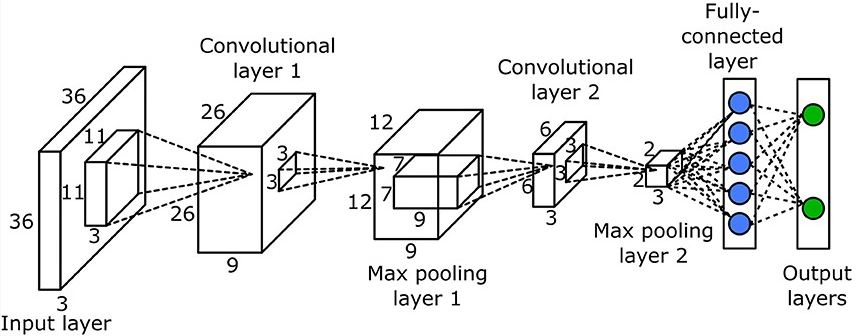
\includegraphics[width=8cm]{CNN}
    \caption{CNN Example}
    \label{fig:CNN Example}
\end{figure}

\section{Definitions}
In this section, different layers of a CNN are explained in detail.
\subsection{\textbf{Input Layer}}
The input to the input layer of the CNN is generally a color image in pixel form which is a three dimensional matrix. The dimensions are length, width and number of channels (R,G,B) of the input image. Generally, the input image is resized to the desired dimensions accepted by the CNN. 

\subsection{\textbf{Convolutional Layer}}
In the convolutional layer, convolution operation happens between the kernel and the input image. Kernel is a 2D array whose elements are obtained from Gaussian distribution. An example of 3x3 Guassian Kernel is given below[2]:
\begin{figure}[h]
    \centering
    \captionsetup{justification=centering}
    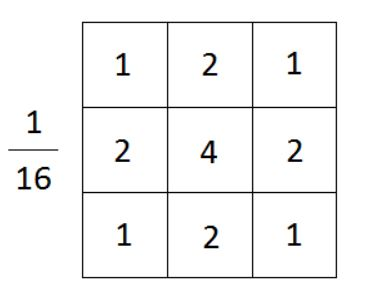
\includegraphics[width=3cm]{Guassian kernel}
    \caption{3x3 Guassian kernel }
    \label{fig:3x3 Guassian kernel}
\end{figure}

Mathematically, 2D convolution is represented as follows:
\begin{equation*}
\boldsymbol{y[i,j] = \sum_{m=-\infty}^{\infty}\sum_{n=-\infty}^{\infty} h[m,n] . x[i-m, j-n]}
\end{equation*}

In convolution layer, the convolution operation is performed on all the pixels by sliding the kernel over the input image. The following image shows the convolution operation between the image and the kernel[3]: 
\begin{figure}[h]
    \centering
    \captionsetup{justification=centering}
    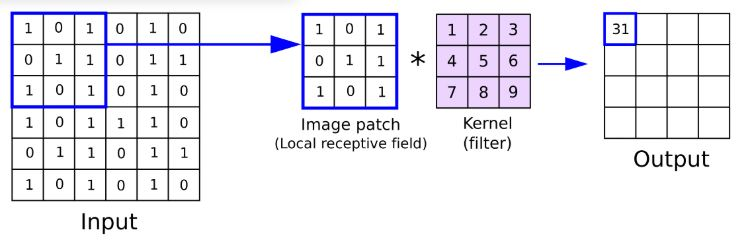
\includegraphics[width=10cm]{conv2d}
    \caption{Convolving kernel over the image}
    \label{fig:3x3 Guassian kernel}
\end{figure}

Typically, in most neural networks the dimensions of the image after performing convolution are maintained same. In order to do that it is important to understand how convolution operation affects the dimensions of the image. The relation is given as follows:
\begin{equation*}
	\boldsymbol{Output Width = \frac{I_W - K_W + 2*P}{S} + 1}
\end{equation*}
\begin{center}
where  $I_W$ is the image width \\
$K_W$ is the kernel width	\\	
P is number of padding bits	\\
S = stride = number of pixels shift over the input image
\end{center}
\begin{equation*}
	\boldsymbol{Output Height = \frac{I_H - K_H + 2*P}{S} + 1}
\end{equation*}
\begin{center}
where  $I_W$ is the image width \\
$K_W$ is the kernel width	\\	
P is number of padding bits
\end{center}

\subsection{\textbf{Pooling Layers:}}
Pooling layers in a CNN is added after the convolutional layer. It reduces the size of the image by retaining only the important features in the image and neglecting the rest. Pooling layers have the following advantages:
\begin{enumerate}
\item It reduces the number of parameters to train in a CNN.
\item It prevents the neural net from over-fitting problem. Over fitting is a situation where the neural net models the training data very well but fails to generalize the results on the testing data. This usually occurs due large number of parameters which lets the neural net detect all the patterns in an image but fails to learn from the patterns to generalize on the testing image. This can be observed when the neural net give more than 95\% accuracy in training data but gives less than 50\% accuracy in testing data.

\textbf{Commonly used Pooling Layers:} Average pooling and max pooling are the two most commonly used pooling layers in neural network.
\begin{enumerate}
\item \textbf{Average Pooling:} In average pooling, the average value is selected from each patch of the feature map to obtained a reduced map size. The following image gives an example of average pooling[4]:

\begin{figure}[h]
    \centering
    \captionsetup{justification=centering}
    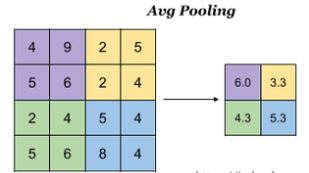
\includegraphics[width=8cm]{avgpool}
    \caption{Average Pooling Example}
    \label{fig:Average Pooling Example}
\end{figure}

In the above example, the feature map is of size 4x4 and the patch is of size 2x2 and stride = 2 and there are no padding bits. So, if we apply the formula for resulting dimension of the feature map, we get the following:
\begin{equation*}
\begin{aligned}
Output Width &= \frac{I_W - K_W + 2*P}{S} + 1 \\
			&= \frac{4 - 2 + 2*0}{2} + 1 \\
Output Width&= 2 
\end{aligned} 
\end{equation*}
\begin{equation*}
\begin{aligned}
Output Height &= \frac{I_H - K_H + 2*P}{S} + 1 \\
			&= \frac{4 - 2 + 2*0}{2} + 1 \\
Output Height&= 2 
\end{aligned} 
\end{equation*}
So, the output feature map will be of size 2x2. Let consider the first (violet) patch and calculate the average pooling output:
\begin{equation*}
Output value = \frac{4 + 9 + 5 + 6}{4} = 6.0
\end{equation*}
This process is repeated over the entire feature map to obtain the reduced 2x2 feature map output.

\item \textbf{Max Pooling:} In max pooling, the maximum value is selected from each patch of the feature map to obtained a reduced map size. Max pooling is the most commonly used pooling layers.  The following image gives an example of max pooling[4]:
 
\begin{figure}[h]
    \centering
    \captionsetup{justification=centering}
    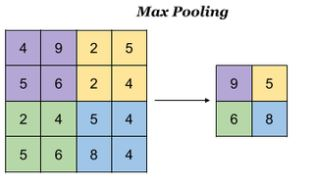
\includegraphics[width=8cm]{maxpool}
    \caption{Max Pooling Example}
    \label{fig:Max Pooling Example}
\end{figure}

As this is the same example used in average pooling, the output feature map size is 2x2. The following i s the max pooling output for the first (violet) patch of the feature map:
\begin{equation*}
Output value = max(4,9,5,6) = 9.
\end{equation*}
\end{enumerate}
\end{enumerate}

\subsection{\textbf{Unpooling Layers:}}
In CNN, inverse operation of pooling layers is not possible. But unpooling layers obtains the approximate inverse of pooling layers by storing the maximum value from each patch of the feature map in a set of switch variables during the pooling operation is being performed. These switch variables  are again in unpooling layers to reconstruct the layer above into appropriate locations. The below picture shows unpooling:

\begin{figure}[h]
    \centering
    \captionsetup{justification=centering}
    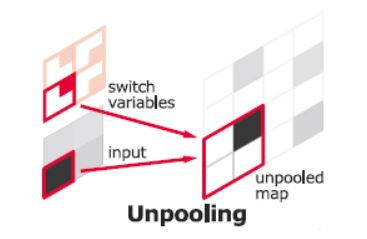
\includegraphics[width=8cm]{unpool}
    \caption{}
    \label{fig:}
\end{figure}
  

\subsection{\textbf{Activation Functions:}}
As the name suggests, an activation function decides whether to activate a neuron or not based on calculating weighted sum and adding bias with it. In the case of a CNN, weighted sum is the output image obtained by convolving the kernel over the input image. Bias is a fixed value which is added pixel wise to the obtained output image. Activation function is applied to this output image which decides whether to select a particular pixel value and pass on to the next layer or not. 
\newline
\textbf{Need for Activation Functions:} In neural networks, the weights (kernel in the case of CNN) and bias values constantly gets updated based on the error at the output. The values are updated using back-propagation algorithm. Activation functions makes the back propagation possible as the gradients are supplied along with errors to update the weight and bias values[5].
\newline
\textbf{Different Activation Functions:} There are different activation functions used in neural networks based on its applications. They are:
\begin{enumerate}
\item \textbf{Step Function:} Step function is a threshold based activation function which outputs 1 for the values greater than a specified threshold or outputs 0 otherwise. Hence, 1 means the neuron gets activated and 0 means neuron gets deactivated. It is shown in the below figure:[7]
\begin{figure}[h]
    \centering
    \captionsetup{justification=centering}
    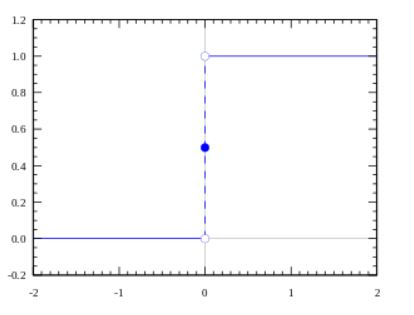
\includegraphics[width=7cm]{step}
    \caption{Step Function}
    \label{fig: Step Function}
\end{figure}
The following conditional equations defines step function:
\begin{equation*}
\begin{aligned}
\text{Activation Function  } A &= 1 \text{    if    } y \geq threshold \\
						&= 0 \text{    otherwise}
\end{aligned}
\end{equation*}
Step function can be used as an activation function if the neural net is being used for binary classification where the output is just "YES" or "NO". Typical example of such classification is determining the picture is of a dog or a cat. 

But, step functions cannot be used as activation functions for multiple(more than 2) classifications as the neural net might give multiple 1's and 0's as output.

\item \textbf{Linear Function:} Linear function means a straight line functions which is proportional to the input. The below figure shows the example:[7]
\begin{figure}[h]
    \centering
    \captionsetup{justification=centering}
    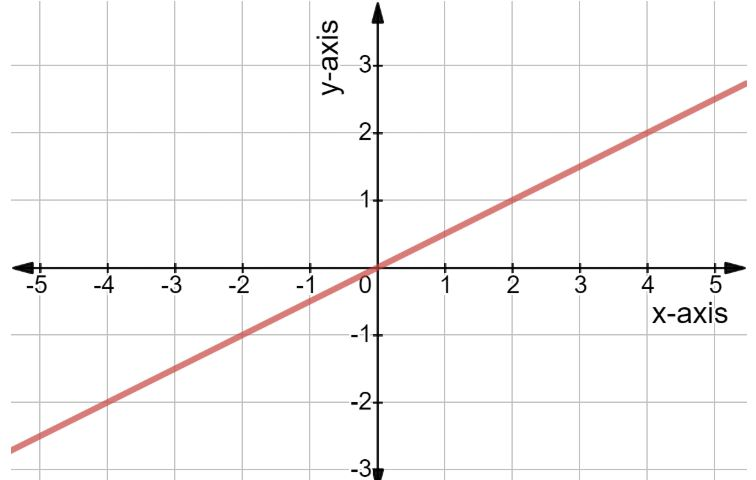
\includegraphics[width=7cm]{lin}
    \caption{Linear Function}
    \label{fig: Linear Function}
\end{figure}
The following conditional equations defines linear function:
\begin{equation*}
\text{Activation Function  } A = c*X
\end{equation*}
Linear function eliminates the multiple classification problem faced by employing step function as the activation function. As the activation function varies with input values, it can take many values not only 0 and 1. Hence, it can classify multiple classes.

The main disadvantage of linear function is the derivative becomes constant. This means that the gradient no longer varies with input. Hence,  if there was an error in detecting the output, since the gradient is constant there will be constant change in the weights and bias values irrespective of inputs. This means that the neural net fails to learn.

Another disadvantage occurs due to linearity property. By, employing linear functions as activation functions to all hidden layers, the output will be a linear combination of hidden layers. Hence, multiple hidden layers can be combined into 1 hidden layer. Hence,  by employing linear function only 1-hidden layer neural nets are possible.
\newline
\item \textbf{Sigmoid Function:} The below picture shows the sigmoid function.[7]

\begin{figure}[h]
    \centering
    \captionsetup{justification=centering}
    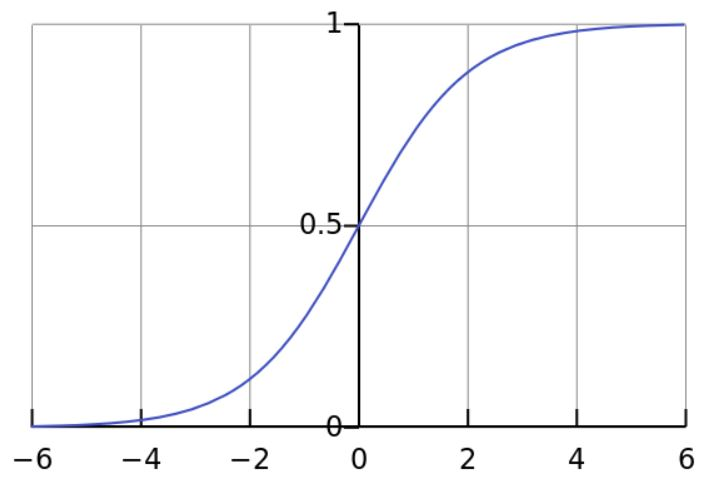
\includegraphics[width=7cm]{sig}
    \caption{Linear Function}
    \label{fig: Linear Function}
\end{figure}
The following conditional equations defines sigmoid function:
\begin{equation*}
\text{Activation Function  } A = \frac{1}{1 + e^{-x}}
\end{equation*}

The sigmoid function is essentially a smoothened version of step function. This makes it far more useful than step function. Firstly, sigmoid function is non-linear which eliminates the linearity problem. Secondly, it can take many values between 0 and 1 which makes it useful in multiple classification problems.

The only disadvantage of sigmoid function is that gradient of the points farther from origin approaches to zero which gives rise to vanishing gradients problem. This makes the neural net to learn very slowly and in worst case scenarios not learn at all.

\item \textbf{Tanh Function:} The below picture shows the tanh function.[7]

\begin{figure}[h]
    \centering
    \captionsetup{justification=centering}
    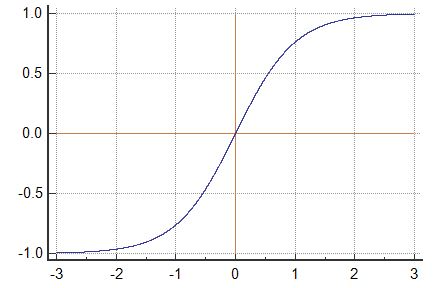
\includegraphics[width=7cm]{tanh}
    \caption{Tanh Function}
    \label{fig: Tanh Function}
\end{figure}
The following conditional equations defines tanh function:
\begin{equation*}
\text{Activation Function  } A = \frac{2}{1 + e^{-2*x}} - 1
\end{equation*}

Tanh function is a scaled version of sigmoid function. The gradient of the points farther from origin approaches slowly to zero than sigmoid function. But, tanh function also faces the problem of vanishing gradient.

\item \textbf{Relu:} Relu stands for Rectified linear unit. It is one of the most commonly used activation function. The figure below shows the function:[7]
\begin{figure}[h]
    \centering
    \captionsetup{justification=centering}
    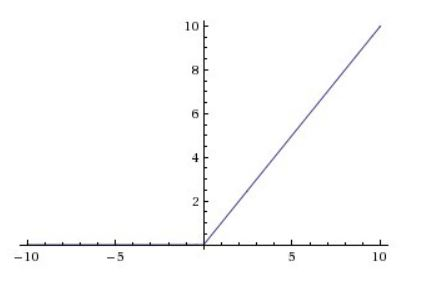
\includegraphics[width=7cm]{relu}
    \caption{Relu Function}
    \label{fig: Relu Function}
\end{figure}

Relu is non-linear in nature as it remains zero for all the negative values for the function which allows neural net to have multiple layers. In addition to this, most of the neurons in the neural net never fire up due to the characteristics of Relu function. This makes the neural net lighter. This makes Relu function less computationally expensive than Sigmoid and Tanh functions.

The disadvantage of Relu function is that for negative values the gradient remains remains zero. This means that some neurons in the neural net will not respond to the change in the output. This is called dying Relu problem.
\end{enumerate} 

\subsection{\textbf{Fully Connected Layer:}}
In neural network, a fully connected later is that layer which connects the inputs of one layer to every activation unit of the next layer. Typically, a fully connected layer is present before the output layer. In a neural net each unit in a convolutional layer contains a feature of the input image essentially an edge. Hence, each convolutional layer is a collection of features of the input image. A fully connected layer holds the composite and aggregate features of all the convolution layers. Hence, a fully connected layer is a feature vector of the input image. The following figure shows an example of a fully connected layer:[8]

\begin{figure}[h]
    \centering
    \captionsetup{justification=centering}
    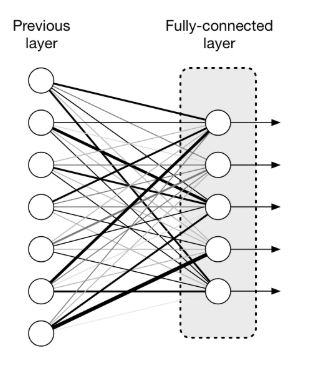
\includegraphics[width=5cm]{fcn}
    \caption{Fully Connected Layer}
    \label{fig: Fully Connected Layer}
\end{figure}

\subsection{\textbf{Deconvolution Layer:}}
Deconvolution layers in CNN is used to represent the output data in the same dimensions as the input image but increasing the size of the output data. Deconvolution is a transpose operation of convolution. 

In deconvolution, first the data is padded and separately according to the desired output size. The below figure shows the representation of data in padded and separated form to convert data of size 2x2 to 4x4:[11]

\begin{figure}[h]
    \centering
    \captionsetup{justification=centering}
    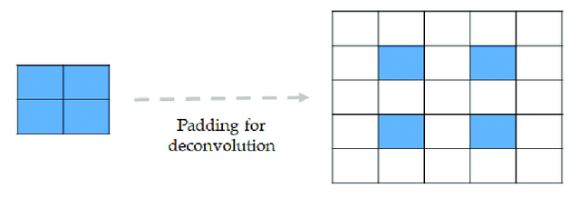
\includegraphics[width=8cm]{deconv1}
    \caption{}
    \label{fig:}
\end{figure}
 
Then the kernel is made to slide over the padded representation to get 4x4 output data size.[12]

\begin{figure}[h]
    \centering
    \captionsetup{justification=centering}
    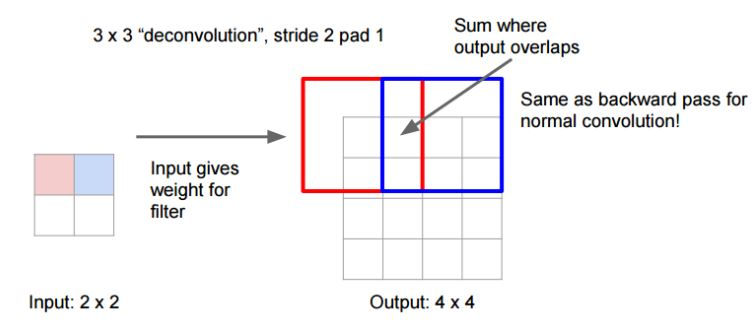
\includegraphics[width=10cm]{deconv2}
    \caption{}
    \label{fig:}
\end{figure}


\subsection{\textbf{Output Layer:}}
The output layer is the final layer of CNN. The output layer takes input from the fully connected layer and assigns probability to it. The assignment of probability is done through softmax activation function. Hence, the output layer outputs the probability of the probability of each class in the input image. The below image shows the softmax activation function present in output layer.[10]

\begin{figure}[h]
    \centering
    \captionsetup{justification=centering}
    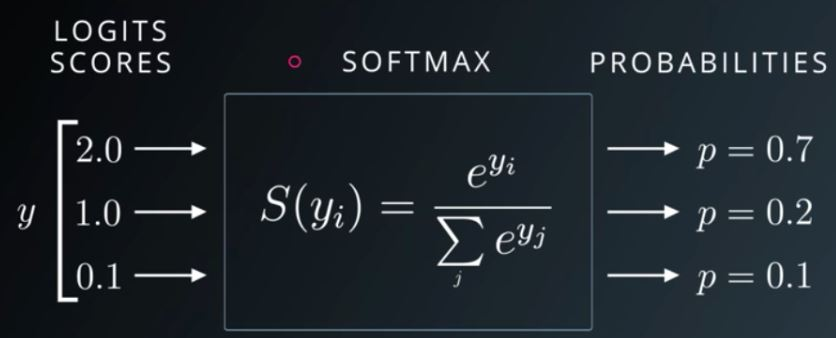
\includegraphics[width=8cm]{softmax}
    \caption{Softmax Activation Function Example}
    \label{fig:Softmax Activation Function Example}
\end{figure}
\newpage
\section{\textbf{U-net Architecture}}
U-net is popularly used CNN for segmentation. The name U-net comes from the fact that the layers in the CNN are arranged in U shape. The below figure shows the U-net architecture:

\begin{figure}[h]
    \centering
    \captionsetup{justification=centering}
    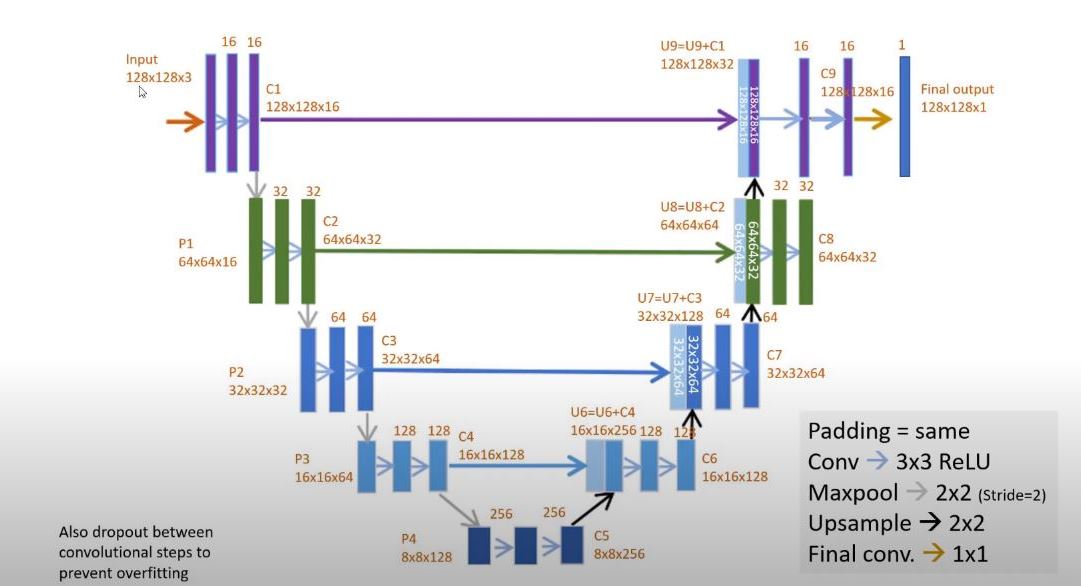
\includegraphics[width=9cm]{u-net}
    \caption{U-net Architecture}
    \label{fig:U-net Architecture}
\end{figure}

The U-net architecture consists of two path. They are:\\
1. Contraction Path: The left half of the U-net where the layers are represented from top to bottom is called contraction path. The contraction path consists of an input layer, sequence of convolution layers, Relu activation layers and max pooling layers. These series of layers reduce the size of the input image simultaneously increasing the number of channels.


2. Expansion Path: The right half of the U-net where the layers are represented from bottom to top is called expansion path. The expansion path consists of sequence of deconvolution or up-convolution layers and concatenation with high resolution features from the contraction path and unpooling layers. The expansion path gives output data in the same size as the input image data. The expansion path increase the size of the contraction path output data simultaneously decreasing the number of channels.



\section{\textbf{References:}}
\begin{enumerate}
\item Layers of a Convolutional Neural Network. (2020, March 02). Retrieved from https://mc.ai/layers-of-a-convolutional-neural-network/

\item MACMAC 51644 silver badges1414 bronze badges. (1969, October 01). Understanding Gaussian Filter and how to plot it in 1-D. Retrieved from https://stackoverflow.com/questions/60462388/understanding-gaussian-filter-and-how-to-plot-it-in-1-d

\item Anh H. Reynolds. (2017, October 15). Convolutional Neural Networks (CNNs). Retrieved from https://anhreynolds.com/blogs/cnn.html

\item Diterbitkan oleh Benny Prijono Lihat semua pos dari Benny Prijono, Prijono, D., Prijono, B., Lihat semua pos dari Benny Prijono, 14, P., Berkata:, P., . . . (wajib), N. (2018, April 03). Student Notes: Convolutional Neural Networks (CNN) Introduction. Retrieved June 26, 2020, from https://indoml.com/2018/03/07/student-notes-convolutional-neural-networks-cnn-introduction/

\item Sakshi TiwariCheck out this Author's contributed articles., Sakshi Tiwari, amp; Check out this Author's contributed articles. (2018, February 06). Activation functions in Neural Networks. Retrieved June 26, 2020, from https://www.geeksforgeeks.org/activation-functions-neural-networks/

\item Intro to Linear vs. Nonlinear Functions. (n.d.). Retrieved June 26, 2020, from https://www.expii.com/t/intro-to-linear-vs-nonlinear-functions-4318

\item V, A. (2017, March 30). Understanding Activation Functions in Neural Networks. Retrieved July 02, 2020, from https://medium.com/the-theory-of-everything/understanding-activation-functions-in-neural-networks-9491262884e0

\item KIDS, T. (2019, July 31). Fully-Connected Layer with dynamic input shape. Retrieved July 03, 2020, from https://medium.com/@tecokids.monastir/fully-connected-layer-with-dynamic-input-shape-70c869ae71af

\item Singh, S. (2019, March 02). Fully Connected Layer: The brute force layer of a Machine Learning model. Retrieved July 03, 2020, from https://iq.opengenus.org/fully-connected-layer/

\item Uniqtech. (2020, April 21). Understand the Softmax Function in Minutes. Retrieved July 03, 2020, from https://medium.com/data-science-bootcamp/understand-the-softmax-function-in-minutes-f3a59641e86d

\item (PDF) A Deep Feature Learning Method for Drill Bits Monitoring Using the Spectral Analysis of the Acoustic Signals. (n.d.). Retrieved July 03, 2020, from https://www.researchgate.net/publication/327007086 A Deep Feature Learning Method for Drill Bits Monitoring Using the Spectral Analysis of the Acoustic Signals

\item Daniil's blog. (n.d.). Retrieved July 03, 2020, from http://warmspringwinds.github.io/tensorflow/tf-slim/2016/11/22/upsampling-and-image-segmentation-with-tensorflow-and-tf-slim/
\end{enumerate}

\end{document}

